\section{Konstruktive Lernverfahren}
Bei allen bisher behandelten Verfahren wird die Architektur des Netzes a priori festgelegt. Während des Trainings wird die Architektur also nicht mehr an das Problem angepasst.\\
Die Idee konstruktiver Lernverfahren ist es, mit einem kleinen Netz zu starten und während des Trainings bei Bedarf weitere Neuronen oder Schichten hinzuzufügen.

\subsection{Upstart-Algorithmus}
Der Upstart Algorithmus konstruiert Binärbäume aus Perzeptronen. Es handelt sich um einen rekursiven Algorithmus zum Erlernen beliebiger binärer Abbildungen mit Schwellwertneuronen.\\

\begin{figure}[h]
    \centering
    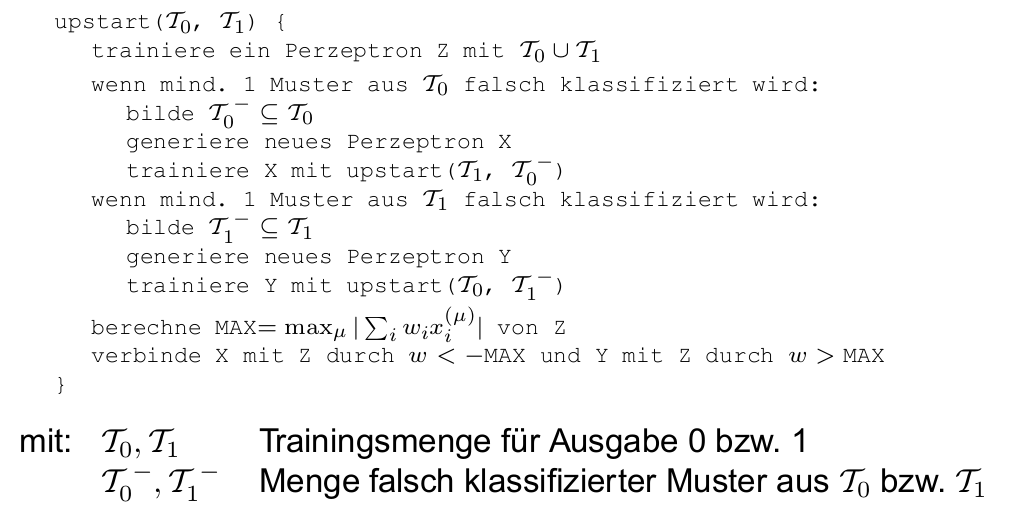
\includegraphics[width=1\textwidth]{img/NeuroLernregel/upstart.png}
    \caption{Upstart Algorithmus}
    \label{ch_lern_upstart}
\end{figure}

\subsection{Cascade Correlation}
\textbf{Motivation}: Bei einem großen Fehler am Ausgang für ein Muster werden alle Gewichte adaptiert. Da es keine Absprache zwischen den Neuronen gibt, kann es vorkommen, dass der Fehler für ein anderes Muster steigt. (\textit{moving target problem}).\\
\textbf{Idee}: Die Gewichte $v_{ij}$ eines verdeckten Neurons $j$ werden separat trainiert, indem die Korrlation zwischen Ausgabe des Neurons und dem Fehler maximiert wird. Danach werden die Gewichte $v_{ij}$ von Neuron $j$ eingefroren, es werden dann weitere verdeckte Neuronen hinzufügt, solange bis der Fehler am Ausgang ausreichend klein ist. 

\begin{figure}[h]
    \centering
    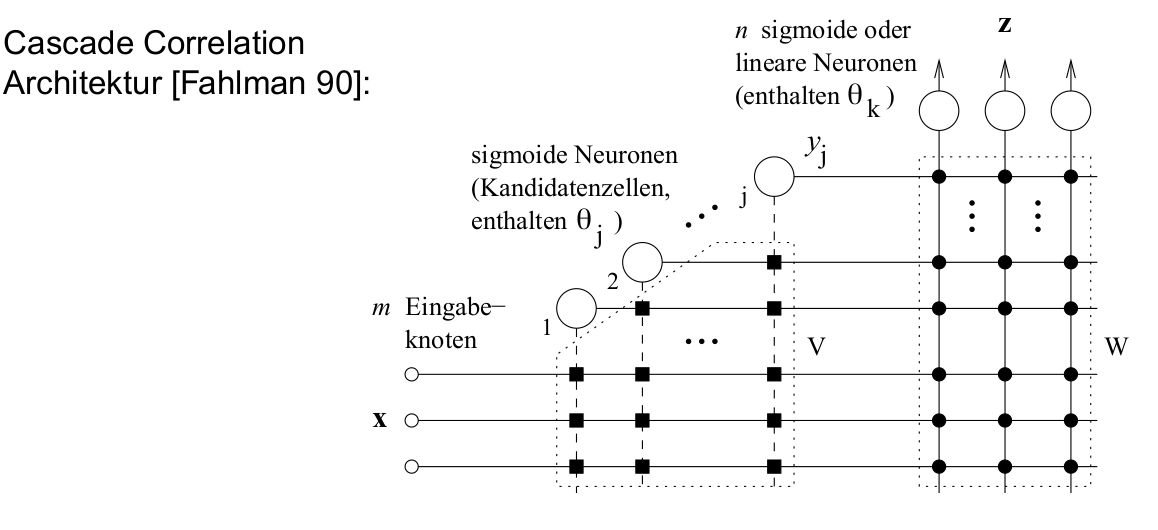
\includegraphics[width=.75\textwidth]{img/NeuroLernregel/cascade_corr_arch.png}
    \caption{Cascade Correlation Architektur}
    \label{ch_lern_cca}
\end{figure}

\todo[inline]{Herleitung der Lernregel (Folie 140/141}

\subsection{Zusammenfassung: Lernalgorithmus für Casecade Correlation}
\paragraph{Schritt (1):}
Trainiere die Gewichte $w_{ik}$ und $\Theta_k$ der Ausgangsknoten mit geeignetem Algorithmus
\begin{itemize}
    \item Perzeptron-Lernalgorithmus
    \item Delta-Lernregel
    \item Quickprop-Verfahren
\end{itemize}
solange bis der Fehler am Netzausgang nicht weiter sinkt.

\paragraph{Schritt (2):}
\begin{itemize}
    \item Stop, falls der Fehler $E$ bereits klein genug ist, sonst
    \item füge ein neues Neuron $j$ hinzu und initialisiere die Gewichte $v_{ij}$ zufällig
\end{itemize}

\paragraph{Schritt (3):}
Bestimme Gewichte  $v_{ij}$ und $\Theta_j$ des neuen Neurons $j$ derart, dass die Korrelation $S_j$ maximiert wird. Adaptiere hierfür $v_{ij}$ und $\Theta_j$ durch Gradientenaufstiegsverfahren, bis Korrelation $S_j$ nicht weiter steigt
\todo[inline]{ausführlicher}

\paragraph{Schritt (4):}
Friere alle Gewichte $v_{ij}$ und $\Theta_j$ des neuen Neurons ein.

\paragraph{Schritt (5):}
Gehe zu Schritt (1)
